% declare documents and packages
\documentclass[man, 12pt, a4paper, noextraspace]{apa6}
\usepackage[T1]{fontenc}
\usepackage[utf8]{inputenc}
\usepackage[american]{babel}
\usepackage{csquotes}
\usepackage{amsmath}
\usepackage{microtype}
\usepackage{caption}
\usepackage{subcaption}
 
\usepackage{graphicx}
\usepackage{url}
\usepackage{times}
\renewcommand{\footnotesize}{\small} % use 11pt for footnotes
\usepackage[doublespacing]{setspace} % single space for footnotes
\setlength{\skip\footins}{1.5pc plus 1pt} % some more space between footnote and main body
% this command put all footnotes to endnote at the end of the paper
%\usepackage{endnotes}
%\let\footnote\endnote

% for word counts
\newcommand{\detailtexcount}{%
  \immediate\write18{texcount -merge -sum -incbib -dir \jobname.tex > \jobname.wcdetail }%
  \verbatiminput{\jobname.wcdetail}%
}
\newcommand{\quickwordcount}{%
  \immediate\write18{texcount -1 -sum -merge \jobname.tex > \jobname-words.sum }%
  \input{\jobname-words.sum} words%
}
\newcommand{\quickcharcount}{%
  \immediate\write18{texcount -1 -sum -merge -char \jobname.tex > \jobname-chars.sum }%
  \input{\jobname-chars.sum} characters (not including spaces)%
}

% Biblatex
\usepackage[style=apa,sortcites=true,sorting=nyt,backend=biber,uniquename=false]{biblatex}
\AtEveryBibitem{%
  \clearfield{issn} % Remove issn
  \clearfield{doi} % Remove doi
  }
% make in-text citations clickable
\usepackage[colorlinks=true]{hyperref}
% this removes annoying colors for in-text citation entries 
\usepackage{xcolor}
\hypersetup{  
    colorlinks,
    linkcolor={red!50!black},
    citecolor={blue!50!black},
    urlcolor={blue!80!black}
}

\addbibresource{abm_misinformation_lit.bib}
\DeclareLanguageMapping{american}{american-apa}
 
\title{If you see something, then say something to others: Complex contagions and the socially-contingent correction of misinformation}

\shorttitle{Socially-contingent corrections}


\author{\addvspace{.25in} Hyunjin Song}

\affiliation{Department of Communication, University of Vienna, Austria}

\abstract{As the citizens' news consumption is increasingly driven by online sources, the propagation of misinformation and so-called \enquote{fake news} on those platforms become an increasing concern for the public and policy makers. Our goal in this contribution is to offer a more systematic assessment of underlying mechanisms of misinformation spreading and its correction, combining a macro social contextual factor and individuals' cognitive basis of adopting misinformation into a more integrated, dynamic system model perspective. We first review existing evidence concerning individuals' cognitive basis of adopting such misinformation, and social context of which exposure to misinformation and its corrections are received. Next, adopting a well-known class of an epidemic model of virus infection and recovery, we combine this micro and macro dynamics into comprehensive, integrated model of misinformation diffusion on social networks. We do so by focusing on the distinction between simple contagion of misinformation vs. complex contagion of adopting corrective messages. Relying on Agent-based simulations, we further explore various boundary conditions of such dynamics, aiming to uncover how and when such misinformation propagates into the public, as well as what factors facilitate or hinder such diffusion process.}

\keywords{Misinformation, fake news, correction, simple contagion, complex contagion, exponential random graph model, agent-based simulations}


\authornote{Hyunjin (Jin) Song is currently an assistant professor ("Universitätsassistent, post-doc") in the Department of Communication at the University of Vienna, and also a member of the Vienna Computational Communication Science Lab.}

\note{Word count: 5339 words \\ %\quickwordcount \\
    Draft date: \today \\
      \addvspace{.25in} 
      \textbf{Draft in progress. Please do not cite without permission.} \\
      Please direct any questions and inquiries to \href{mailto:hyunjin.song@univie.ac.at}{hyunjin.song@univie.ac.at}}

\begin{document}
\setcounter{page}{0}
\maketitle
  Citizens across the worlds are experiencing major changes in their news environments with the development of digital media. One of the most dramatic changes in the news environment in recent decades involves the role social networking sites (SNS) such as Facebook and Twitter play as a primary source of news outlets. Not only citizens' news consumptions are increasingly driven by such online sources \parencite{shearer2017news}, but it also appears that citizens themselves are actively participating in news dissemination on those platforms by sharing news contents with their peers \parencite[e.g.,][]{shearer2017news, lee2017people}. 

  An effective deliberation among public is regarded as a keystone of thriving democracies, and modern political systems squarely depend  on  informed  decisions of citizens in that regard \parencite{carpini1996}. Yet, a propagation of rumors, misinformation, and so-called \enquote{fake news} on those platforms becomes an increasing concern for the public and policy makers alike \parencite{allcott2017social, lazer2017combating}, as evidenced in recent 2016 U.S. presidential election \parencite{guess2018selective, giglietto2016fakes, allcott2017social} and in Brexit votes \parencite{nyt_2017}. While a wide circulation of factually dubious information is not entirely new to political arena, a growing trend of digitally disseminated rumors and misinformations -- often termed as a \enquote{fake news} phenomenon -- is increasingly recognized as a serious threat to liberal democratic societies \parencite{allcott2017social, lazer2017combating}. Either based on unsubstantiated rumors or based on factually wrong beliefs, many of the misinformed behave differently than those who are accurately informed \parencite{kuklinski2000misinformation}. They often disagree about basic facts about many public issues, and continue to believe and rely on such false information when making political judgments \parencite{nyhan2010corrections,thorson_2016}. 

  Along with these trends, there has been an growing interest among scholars on how people process and maintain factually false (or at least factually dubious) information from the perspectives of an individual's cognitive processes \parencite{Lewandowsky_2012PSPI, kuklinski2000misinformation, weeks2015emotions}. These studies have generated a valuable insights of how individuals often maintain factually false beliefs, and further, how corrections to false beliefs are received and processed \parencite{Lewandowsky_2012PSPI, thorson_2016, garrett2016driving}. However, despite growing interest and continued research effort to better understand the nature and its exact mechanism, what we know about the spread of misinformation and fake news specifically on online social networks is largely based on limited evidence due to its complex nature of the problem.

  Against this backdrop, our goal in this contribution is to offer a more systematic assessment of underlying mechanisms of misinformation spreading and its correction, focusing on one's \emph{social contexts} in which such (mis)information and corrective messages are received and processed. We argue that while \emph{exposure} to (mis)information is likely to follow a simple contagion process, \emph{changes} in one's beliefs regarding such (mis)information -- which ultimately \emph{the} goal of corrective messages -- is likely to be, in \citeauthor{centola2007complex}'s (\citeyear{centola2007complex}) term, a \enquote{complex contagion} where such changes require multiple sources of affirmation and reinforcement compared to simple contagion process. As a result, the effects of fact-checking and corrective messages are likely to be highly \emph{socially} contingent, yet studies only now begin to consider this possibility more seriously \parencite{margolin2017, bode2017see}.    
    
  In what follows, we first review existing evidence regarding political misperceptions and the effects of fact-checking (i.e., correction) messages. We advance our perspective by combining an individual-level cognitive and affective basis of adopting such misinformation with a social context of which misinformation and corrections are received. Based on a well-known class of an epidemic model of virus infection and recovery, we propose an integrated model of misinformation diffusion and socially-contingent corrections on social networks, with a special focus on the differences between a \emph{simple contagion} of misinformation and a \emph{complex contagion} of corrections and fact-checking messages. Relying on Agent-Based Model (ABM) simulations, we robustly explore boundary conditions of such dynamics, aiming to uncover how and when such misinformation propagates into the public.
    
\section{Psychological Underpinnings of Fake News, Misperceptions, and Corrections}

     Following \citeauthor{allcott2017social}'s (\citeyear{allcott2017social}) definition, we define \emph{fake news} as \enquote{distorted signals uncorrelated with the truth} (p. 212). This encompasses several related concepts, such as misinformation, rumors, and disinformation. Literature on this topic generally maintain loosely defined, but at the same time highly interrelated, conceptualizations of those related terms. For instance, (political) rumors are often defined as \enquote{unsubstantiated claims about candidates and issues that are often false} \parencite[p. 401]{weeks2014electoral}. Similarly, misinformation (or misperceptions) are defined as factual information (or beliefs) \enquote{that are false or contradict the best available evidence in the public domain} \parencite[p. 128]{flynn2017nature}. In relation to this, \emph{dis}information campaigns often denote organized, strategic efforts that trying to sway public opinion using rumors and misinformation \parencite{Garrett2017distraction, Lewandowsky_2012PSPI}. Understood in this way, fake news often exclude unintentional reporting mistakes, parodies and satires, or unverifiable conspiracy theories \parencite{allcott2017social}. While term \emph{fake news} often than not additionally entail specific pseudo-journalistic styles that mimic legitimate news sources to intentionally deceiving audiences \parencite{jana_sophie_fn}, we use term \enquote{fake news} somewhat loosely, denoting any type of misinformation -- information that is not supported by best-available evidence -- that is deliberatively circulated among publics.\footnote{  Often, the term \emph{fake news} is used as derogatory, rhetorical label to attack political opponents. While such a use of the term as a \emph{label} is an important conceptual dimension to consider, this aspect of \emph{fake news} is beyond the scope of this manuscript. See \citeauthor{jana_sophie_fn} (\citeyear{jana_sophie_fn}) instead for a detailed conceptualization involving this distinction.}
     
      Literature on misinformation and its persistence often converges to the observation that publics' exposure to and acceptance of misinformation are largely driven by one's motivated consistency needs. That is, people disproportionately gravitate toward information that conforms to their partisan priors \parencite{ weeks2014electoral, garrett2016driving}, and  more likely to accept and endorse such messages \parencite{nyhan2010corrections, guess2018selective}. A mounting evidence -- largely based on \citeauthor{kunda1990}'s (\citeyear{kunda1990}) or on \citeauthor{taber2006}'s (\citeyear{taber2006}) motivated reasoning framework -- suggests that citizens tend to evaluate attitudinally congruent information as more convincing and valid \emph{regardless of its veracity}, while attitudinally inconsistent information is likely to be perceived as weak and therefore likely to be rejected. Therefore, it is perhaps not surprising to find that most of the prior studies based on a motivated reasoning framework document that fact-checking messages (sometimes denoted as \enquote{corrective} or \enquote{debunking} messages in the literature) have only limited effects due to inherent tendency of humans to directionally process politically relevant information \parencite{thorson_2016, taber2006,flynn2017nature}. Even worse, corrective messages may backfire, may induce higher level of endorsements of false beliefs than actually lower them \parencites[e.g.,][]{nyhan2010corrections}[but see][]{Wood2018}.
      
      Another line of studies based on a dual process theory of human cognitive processing and memory suggests that attitudinally-congruent misinformation creates automatic and strong affective responses -- therefore automatically and effortlessly activated in one's memory -- whereas attitudinally incongruent correction messages rarely produce such responses. Due to such asymmetrical nature, people have to rely on more deliberative, strategic search processes (which require significant cognitive resources) to recall attitudinally inconsistent correction messages and incorporate them into relevant judgments \parencite{thorson_2016, Lewandowsky_2012PSPI}. Also, since misinformation tends to form a coherent mental model based on one's partisan schema and stereotypes \parencite[e.g.,][]{garrett2013undermining}, people tend to fill any gaps caused by corrections (that invalidate some parts of the existing mental model) with flawed but attitudinally congruent misinformation that is still readily accessible in their memory \parencite{Lewandowsky_2012PSPI}. Studies also find that this effect is much more likely when correction messages do not update the initial mental model that justifies misinformation \parencite{Chan_debunking_meta_2017}, when the perceived veracity of initial misinformation is high \parencite[due to fluency bias in one's cognitive processing:][]{Lewandowsky_2012PSPI}, or when individuals can generate counter-arguing reasons in support for initial misperceptions \parencite{garrett2013undermining, Chan_debunking_meta_2017}. Most importantly, due to limitations of strategic memory search processes (i.e., it requires more effortful processing), people may still rely on negated misinformation in subsequent reasoning \emph{even when they remember such information is factually incorrect} \parencite{Lewandowsky_2012PSPI}. Therefore, even in the face of seemingly effective corrections, the effect of misperceptions lingers and continue to exert influence \parencite{thorson_2016}.  
      
  Under certain situations, it seems that citizens \emph{indeed} can adhere factual information based on correction messages despite their perpetual partisan bias \parencite[e.g.,][]{Wood2018, nyhan2017taking}. Yet as \citeauthor{margolin2017} (\citeyear{margolin2017}) note, it appears that such effects often require special \emph{social context}. This observation is indeed much warranted, as most of the previous studies concerning misinformation and the effect of fact-checking messages are conducted in an experimental context with a single-shot, \emph{asocial} correction message from media professionals and fact-checking organizations \parencite[e.g.,][]{nyhan2010corrections,garrett2013undermining,weeks2015emotions}. Much of the literature on partisan selective exposure and political discussion networks already point that social contexts of which an individual is exposed to counter-attitudinal messages may have a powerful consequence on how such messages are interpreted and processed \parencite{messing2014selective, levitan2008resistance}. There is also a suggestive evidence that fact-checking and corrective messages from one's peers in their social networks -- what we would call a \enquote{social correction} -- are more likely to, if not equally, be effective in reducing misperceptions \parencite[e.g.,][]{margolin2017, bode2017see}. In what follow, we review several theoretical accounts of such \emph{socially-based} correction messages on misinformation and fake news.   
      
\section{A Social Context of Misinformation and Corrections: Simple vs. Complex Contagions}

  People's perceptions and behaviors are likely to be shaped by their social contacts \parencite{lazer2010coevolution, centola2007complex}, and therefore perceptions and behaviors may spread within social networks \parencite[e.g.,][]{bond_61million}. Indeed, a non-negligible number of prior accounts of partisan misinformation and fake news on social networks connects this idea to possible mechanisms of misinformation propagation and \emph{spreading}  \parencite[e.g.,][]{del2016spreading, Bakshy_2012}. The most simplest form of those accounts posits that online social networks provide one of the ideal settings for partisan misinformation and fake news to be spread within such networks. Many of the partisan rumors and fake news tend to be richer in their \enquote{novelty} \parencite{wu2007novelty} regardless of its veracity and informational value. As \citeauthor{giglietto2016fakes}'s (\citeyear{giglietto2016fakes}) observation suggests, such non-redundant and \enquote{novel} information (false and unverified information being one of them) tend to be engaging, and spread faster via weaker ties \parencite{granovetter1977strength}. You can easily share and post such news with little to no effort, and your friends on your social networks are easily exposed to such information, in turn they also share such news to their own peers, and so on -- creating what is called a \emph{information cascade} of misinformation \parencite{del2016spreading}. Also, individuals maintain lots of weak ties in social network platforms, which is thought to diversify the information flow. This creates a particularly congenial scenario for a (mis)information propagation and dissemination \parencite{Bakshy_2012, granovetter1977strength}. Indeed, \citeauthor{guess2018selective}'s (\citeyear{guess2018selective}) investigation of fake news consumption during the 2016 U.S. presidential election suggests that Facebook was likely to be the focal gateway for visiting websites that propagates fake news, while \citeauthor{allcott2017social}'s (\citeyear{allcott2017social}) study also reveals that such dubious stories are indeed widely shared on Facebook during the election. 
    
    Often, this process of spreading (mis)information within a social network can be described as a \emph{simple contagion} process -- the process of which a single contact with an \enquote{infected} individual (in this case, those who spread misinformation to their peers) is sufficient for such misinformation to be spread to another individual \parencite{Monsted_plos2017, Centola2010Sience, siegel2009social}. While a spread of any human behavior requires a minimum threshold of one, for the diffusion of information itself -- much like communicable diseases -- \enquote{the threshold is almost always exactly one}  \parencites[][p. 706]{centola2007complex}[also see][]{Centola2010Sience}. Once your peer shares news, you become (almost automatically) aware of such news, and you do not require someone else to keep asking about the same news in order to be \emph{aware} of it.  
    
    Moreover, due to inherent partisan motivated directionality, the threshold of actually \emph{adapting} such a false yet pro-attitudinal claim (i.e., believing attitudinally congruent misinformation) may also exhibit similar low-threshold properties, although the actual threshold for believing misinformation would be bit higher compared to that of mere exposure and awareness \parencite[e.g.,][]{Monsted_plos2017}, and also subject to some individual differences \parencite[e.g.,][]{weeks2015emotions, flynn2017nature}. As previously suggested, people tend to directionally process political information \parencite{taber2006}, and they tend to easily remember and recall attitudinally-consistent information than uncongenial ones. Therefore, at least for citizens who find given misinformation to be congenial to their partisan priors, \emph{adapting} such false yet pro-attitudinal claims also does not require high number of repeated exposure nor independent, multiple exposure to different sources supporting such claims. Indeed, many of the prior empirical studies support this perspective \parencite[e.g.,][]{garrett2016driving, kuklinski2000misinformation, flynn2017nature}.         
    
    In contrast, there are reasons to believe why the effectiveness of fact-checking and corrective messages would be different from that of a simple contagion of misinformation. An adoption of a new perspective that contradicts with one's priors (such as an adoption of counter-attitudinal fact-checking messages) is likely to be, in \citeauthor{centola2007complex}'s (\citeyear{centola2007complex}) term, a \enquote{complex contagion} where it requires \emph{exposure to multiple sources}, rather than \emph{multiple number of exposures}, endorsing such message in order to be accepted and further spread into a given network. This is because many political attitudes and subsequent actions (such as politically motivated misperceptions) are likely to be deeply rooted in one’s social identities and values, therefore changes in one's political beliefs and attitudes require multiple sources of affirmation and reinforcement from multiple \emph{contacts} compared to simple contagion cases \parencite[e.g.,][]{gonzalez2017decoding, larson2016social, siegel2009social}. 
    
    Moreover, such complex contagion dynamics surrounding correction messages are also likely to be dependent upon the attitudinal composition of one's local network. For the case of a adoption of fact-checking and corrective messages, the number of one's neighbors who are \emph{not} activated (e.g., those who still \emph{endorse} false belief based on misinformation) tend to discourages their neighbors to adopt a correction, whereas the number of one's neighbors who are already activated (e.g., those who do not believe misinformation anymore) would increase one's susceptibility to adopt the correction given exposure to such correction \parencites[i.e., a \enquote{\emph{contested}} contagion:][]{centola2007complex}[also see][]{friedkin2001norm}. Indeed, many social contagions are often perceived to be lack of credibility and legitimacy until adopted by one's neighbors, therefore relative distribution of one's neighbors (in terms of supporters vs. opponents of the adoption) critically influence one's decision to adopt a controversial innovation \parencite{larson2016social, gonzalez2017decoding, friedkin2001norm}. This further means that locally-defined social dynamics may drive specific adoption behaviors of counter-attitudinal information, and consequently, such process would non-trivially interact with a structure and its attitudinal composition of a given network \parencite[e.g.,][]{friedkin2001norm}. Indeed, there exits a considerable support for this perspective, such that different network topologies \parencite[][]{Centola2010Sience, siegel2009social} or attitudinal makeup of social networks\footnote{  Here, we use the term \enquote{attitudinal composition} to denote a relative distribution of supporters vs. opponents regarding a given attitude or a behavior being spread in a network.} \parencite[][]{levitan2008resistance, larson2016social, gonzalez2017decoding} may produce different attitudinal and behavioral consequences for social influence. This further implies that some network structures are more prone to generating cascades and adoptions than others.

  There are also at least several other reasons why socially-based correction messages, especially from one's peers, might be more effective than a single-shot, \emph{asocial} correction message from more distanced sources (such as fact-checking organizations or mere strangers). First, people may evaluate information coming from their peers to be more credible and trustworthy \parencite[e.g.,][]{metzger2010social}, and more willing to deliberate with their close social contacts \parencite{morey2012matters}. Research suggests that while individuals rather maintain much flexible attitudes as long as their social affiliation goals are met \parencite{levitanspy2017}, reputational risks and social accountability of rejecting corrective messages run high for more close social contacts compared to more distant sources such as strangers \parencite{margolin2017}.  
    
    Second, previous studies concerning citizens' political discussion network suggest that an individual's network construction is not likely driven by overt partisan considerations \parencite{song2015uncovering,lazer2010coevolution}, therefore there exists a considerable degree of exposure to disagreement in citizens' everyday political interactions \parencite[e.g.,][]{Bakshy1130, morey2012matters}. Under such a situation, attitudinally heterogeneous networks trigger more systematic processing of available information, which make individuals to be more responsive to argument strengths \parencite{levitan2008resistance} or social utility \parencite{messing2014selective}, therefore makes them less resistant to corrective messages from their peers.    

  All in all, prior empirical evidence and theoretical perspectives convincingly suggest that a \emph{simple} contagion of misinformation and a \emph{complex} contagion of corrective messages would exhibit different properties for population-level propagation dynamics. Structurally weak, but bridging ties such as distant contacts in social networks may provide sufficient means for a simple (mis)information -- much like communicable disease -- to be spread, while ideologically-driven directionally motivated reasoning may provide sufficient psychological grounds for partisans to easily adopt and believe such misinformation. In contrast, an adoption of corrective message -- similar to controversial innovations -- requires independent and multiple reinforcements from many social contacts due to its counter-attitudinal and \enquote{contested} nature, critically dependent upon a structure of network and its attitudinal composition \parencite{centola2007complex, Centola2010Sience, gonzalez2017decoding}. Aforementioned perspectives therefore undoubtedly point to the possibility that adoptions of fact-checking messages are likely to be highly socially-contingent, and under certain cases, a social correction would be much more effective than an isolated correction message as typically have been considered in previous experiment contexts \parencite[e.g.,][]{nyhan2010corrections,garrett2013undermining}.
    

\section{Observational Challenges in Studying Misperception Within Social Networks}

  If the diffusion of (mis)information and adoption of corrective messages may non-trivially dependent upon a structure of a given network and its attitudinal composition, then how a typical (online) social network is structured in terms of its topological features, and how pervasive is \enquote{attitudinal} homophily, as \emph{the} critical factor determining attitudinal compositions, on such a social network? How such structural features affect the overall diffusion dynamics empirically? This is indeed important questions to ask, since the flow of information (either misinformation or its correction) and its adoption are ultimately structured by how individuals are connected with each other in a given network. However, it is surprisingly difficult to establish convincing evidence of the impact of structural properties of a given network and its attitudinal composition in complex contagion dynamics using purely observational and experimental approaches.
    
    A frequent and recurring theme for an attitudinal makeup of citizens' social networks and its consequences, especially among general publics, is that most of the citizens today are put into a \enquote{echo chamber} or a \enquote{filter bubble} that insulate themselves from competing viewpoints and attitude-discrepant information \parencite[e.g.,][]{lewandowsky2017beyond, del2016spreading}. Yet, as \citeauthor{Garrett2017distraction} (\citeyear{Garrett2017distraction}) puts it, \enquote{there is ample evidence that \emph{exposure} [emphasis added] echo chambers are not a typical part of Internet users' experience} (p. 370). Most of citizens are appear to be embedded in sufficiently diverse social networks, showing a substantial level of exposure to political difference in online \parencite[e.g.,][]{Bakshy1130, messing2014selective} and in offline \parencite[e.g.,][]{huckfeldt2004disagreement}. More importantly, those studies do not find compelling evidence that ordinary citizens' network constructions are primarily driven by purposive political homophily that limit their exposure to only congenial political perspectives \parencite{song2015uncovering, lazer2010coevolution}. This suggests that popular claims of echo chambers or filter bubbles are often overstated.\footnote{    Indeed, in a completely segregated network where cross-ideological links are not present, a simple diffusion of partisan misinformation is not likely to saturate the entire network, since at least some segments of populations are never exposed to such information due to the lack of cross-ideological exposure. In light of our discussion, an \enquote{exposure} echo chamber actually \emph{prohibits} global-scale (mis)information propagation.} 
    
    However, one should also bear in mind that the evidence concerning \emph{exposure} to counter-attitudinal messages does not provide sufficient evidence of how such messages are actually cognitively processed and interpreted under such a situation \parencites[e.g., see "engagement echo chamber" discussion in][]{Garrett2017distraction}[also, see][]{nyhan2017taking}. What we know about citizens' exposure to disagreement in their social networks typically has relied on observational evidence, either based on participants' self-reports of their patterns of social interactions concerning their immediate social environment \parencite{huckfeldt2004disagreement} or based on a comprehensive mapping of their interactions in a well-defined, relatively closed social system \parencite[e.g.,][]{song2015uncovering, lazer2010coevolution}. Sometimes, scholars also rely on digitally available communication patterns such as messages posted in online social networks \parencite[e.g.,][]{margolin2017}, along with engagement indicators such as \enquote{likes} or \enquote{shares} \parencite[e.g.,][]{Bakshy1130} or based on a detailed digital footprint data such as website access data \parencite[e.g.,][]{guess2018selective}. While such evidence \emph{do} suggests that citizens are indeed frequently exposed to competing political perspectives in their daily lives, such evidence is typically rather silent about how individuals actually process and interpret such information given exposure. As experimental evidence to date suggests, the mere presence of ideologically diverse \emph{exposure} does not automatically translate into the possibility of more balanced judgments. Experimental evidence in this regard can provide more detailed pictures of how such (counter-attitudinal) messages are actually selected, processed, and adopted by an individual given exposure settings \parencite[e.g., ][]{messing2014selective, nyhan2017taking, Wood2018}. Yet as previously suggested, a typical experimental approach tends to be misspecified in terms of crucial social dynamics surrounding simple vs. complex contagion of misinformation and correction messages within a naturally-occurring social network \parencite{margolin2017, Centola2010Sience}. Moreover, designing a realistic experiment involving real-world social interactions often involves significant practical \parencite[e.g.,][]{bond_61million} and ethical challenges \parencite[e.g.,][]{Kramer8788} for researchers.       
    
    Similarly to attitudinal composition of citizen's social networks, the question of how exactly the structure of citizens' social networks exhibits certain topological properties have attracted considerable interests among scholars. Prior observations on this topic suggests that large-scale (online) social networks tend to exhibit \enquote{small-world} like properties \parencite{kumar2010structure, ugander2011anatomy}. A small world is characterized by its typical structure where most nodes can be reached from every other nodes by a small number of steps compared to a pure random graph of the same size. This is due to the fact that a small minority of \enquote{hub} nodes posses a disproportionate number of links, providing a global bridge between smaller, more strongly interconnected local clusters \parencite{barabasi2004linked}. 
    
    This structure has traditionally been known for information to be spread globally through such hubs \parencite[e.g.,][]{Bakshy_2012}, following \citeauthor{granovetter1977strength}'s (\citeyear{granovetter1977strength}) seminal account of strength of weak ties. However, emerging evidence suggests that such a small-world structure may hinder a given diffusion process to globally saturate the network, since such hubs can serve as a \enquote{bottleneck} of a contagion process, therefore diffusions are stay localized and compartmentalized \parencite[e.g.,][]{banos2013diffusion, centola2007complex, zhao2010weak}. Similarly, while the existence of tightly-knit neighborhoods in a typical small-world network supports a complex-type behavioral propagation \parencite[i.e., an innovation that runs counter to prevalent norms and values:][]{Centola2010Sience}, the existence of hubs may not favor complex contagion to be globally propagated into a given network. This is due to the fact that such hubs require a much higher number of active neighbors to meet the threshold of adopting a controversial innovation (i.e., complex contagions), and even if such hubs are activated, they alone cannot further activate their immediate neighbors to adopt such  innovations in the absence of other local nodes that provide multiple independent reinforcements \parencite{Centola2007449, zhao2010weak, gonzalez2017decoding}. Therefore, whether topological properties of a given network actually hinder or facilitate a contagion process may critically dependent upon specific thresholds values for complex contagions and its interaction with the structure of network \parencite[e.g.,][]{Centola2007449}, which is often hard to be tractable empirically.   
    
    Moreover, especially for the case of misinformation and its corrections, a simple contagion (of misinformation) and a complex contagion (of correction messages) may simultaneously affect a local-level attitudinal composition of one's neighbors \parencite[i.e., those who endorse and believe misinformation vs. those who do not: e.g.,][]{campbell2013complex}. Last but not least, all of aforementioned factors are endogenously determined through prior states of networks over time in evolving dynamic network. As a consequence, a proper identification regarding the exact impacts of its attitudinal composition and structural properties of an given network often necessitates systematic comparisons between the observed network and a number of plausible counterfactuals. Doing so further requires (a) the ability to compared different thresholds values for complex contagions, and (b) the ability to independently manipulate topological structures of a social network \parencite[e.g.,][]{Centola2010Sience, Centola2007449, gonzalez2017decoding}. For this reason, a rigorous empirical test of such factors is often practically impossible for observational studies despite its scientific and practical importance. 
    
\section{A Current Investigation: Mathematical Modeling of Complex Diffusion Dynamics}

  Adopting a well-known class of an epidemic model of virus infection and recovery, this study used stochastic network-based mathematical models to simulate contagion dynamics of misinformation and its corrections. More detailed methods, including model parameterization, simulation, and more detailed analyses of simulation model results, are provided in the supplementary appendix. Behavioral parameters governing the network structure and misinformation propagation dynamics were estimated from several best-available existing nationwide representative surveys concerning citizen's social network \parencite[American National Election Study 2008–2009 Panel Survey:][]{ANES2009} and exposure to fake news during 2016 presidential election \parencite{pewfakenews}. Although these data sources were not specifically designed for obtaining the impact of (mis)information diffusion dynamics within a social network but rather conveniently chosen,\footnote{  It should be acknowledged that those sources of data is suboptimal in number of regards: (a) social network data is confined to cross-sectional, egocentric network data, and (b) they do not come from the identical data generating process covering the same periods of observations (e.g., networks recoded in 2009 has little or no bearing for fake news exposure in 2016). However, research indicates the structural compositions of citizens' core discussion network are reasonably stable over time, albeit actual responses in typical surveys are subject to a number of survey-context related factors \parencite{byungkyu2017important} or changes in one's life contexts \parencite{small2015stable}. Also, since most of the prior applications concerning fake news and misinformation from observational studies typically look at representative samples, we intentionally have chosen those data since these types of data are more commonly used in the social sciences, which provide best-available up-to-date relevant information for the current application. See also \textit{A Stochastic Dynamic Model of Networks} section below and supplemental appendix for a detail.} it nevertheless provides reasonable starting point for formally model more realistic network structures, on which we later further parameterizing the assumptions and mechanisms postulated in the previous discussions of complex diffusion dynamics. All simulation models were based on the \emph{EpiModel} R software package \parencite{epimodel}.
    
    Utilizing simulation-based approach in modeling (mis)information propagation is not entirely new \parencite[e.g.,][]{tambuscio2015fact, jin2013epidemiological, acemoglu2010spread, zhao2010weak}. Yet these studies have typically relied on a series of deterministic compartmental models, where diffusion dynamics were derived by differential equations representing analytic epidemic systems \parencite[e.g., see][]{zhao2010weak}. While they offer valuable insights of how information spread in a given system, they do not explicitly represent contact phenomena in a network, therefore somewhat limited in realistically representing the evolving dynamic networks on which information and behaviors are spread conditional on the network structure. Our approach was to use an exponential random graph model, or ERGM framework \parencite{robins2007introduction, morris2008specification}, to simulate a series of dynamically evolving networks of different topological properties (see also below section XXX for a more detail). The ERGM framework is now regarded the most versatile yet flexible method for identifying how a given network is formed and evolves based on the underlying generative principles \parencite{cranmer2017navigating, robins2007introduction}, and for a simulation context, it offers a convenient yet powerful tool for independently manipulating topological structures of a network based on such generative mechanisms by a researcher's choice \parencite{morris2008specification, leifeld2017temporal}. In our present application, we therefore simulated a baseline model (based on available empirical evidence) and several counterfactual models (that differ in some key parameters) of network evolution models, and further submit them to different stochastic models of misinformation propagations vs. corrective message adoptions. Our focus here is therefore on the role of varying level of attitudinal homophily as a driving force of network evolutions, and how attitudinal compositions of one's local networks (as end-results of attitudinal homophily) interactively influence simple vs. complex contagion dynamics at population level in conjunction with network topologies.
    
    Therefore, our approach differs from prior studies that have used similar simulation-based approaches in three critical aspects: (a) instead of relying on purely hypothetical scenarios and parameter values, we augment our model by supplying more realistic parameter values based on existing empirical evidence; (b) our model explicitly takes into account the stochastic nature of network evolution and its endogenous influence over time; and finally, (c) we explicitly model how attitudinal compositions of one's immediate neighbors and local-level contagion dynamics (i.e., simple vs. complex contagions) interact to yield propagation dynamics at the population level. Arguably, this approach obviously still greatly simplifies the complexity of the real world. However, in doing so, it provides an analytical tool for identifying the effects topologies and attitudinal compositions of a network, and the resulting implications for the simple vs. complex diffusion dynamics of misinformation and corrections in a typical social network.

\subsection{A Stochastic Dynamic Model of Networks}

  In order to explore role of network topologies in diffusion dynamic in evolving networks, we require to explicitly specify a network structure and how such structure evolves over time according to some underlying generative principles. To this end, we first model formation and dissolution of citizens' political discussion ties over time (through which misinformation and corrections are communicated) using separable temporal ERGMs (STERGMs), using \enquote{summary statistics} drawn from egocentric network samples \parencite{krivitsky2017inference}. That is, we estimate and simulate \emph{complete networks} that consistently reproduce observed properties of egocentrically sampled information from 2009 ANES data.\footnote{ Of course, this approach requires certain assumptions in order to define a model that represents a distribution of networks that are centered on the observed properties. See \citeauthor{krivitsky2017inference} (\citeyear{krivitsky2017inference}) for a detailed discussion of this class of models and their properties.} Those observed properties, or summary target statistics, include: density (i.e., average number of discussion partners, or \enquote{alters}), average expected number of degrees among Democrats and Republicans excluding Independents (i.e., main effect of partisanship), the extent of partisan homophily (i.e., interaction between ego and alter partisanship), and number of people who posses multiple contacts (i.e., degree distributions).\footnote{  In 2009 ANES panel, there are a total of 1258 self-identified Democrats and 1142 self-identified Republicans (including respective party leaners), excluding 336 Independents. Those 2400 partisans (i.e., Democrats plus Republicans) have on average 1.975 discussion partners. Since in 2009 ANES respondents theoretically name up to three alters, this translate into egonetwork density of 0.66 (=1.975/3). For the main effect of partisanship, the marginal distribution of number of named alters by egos did not differ by partisanship, meaning that the expected mean degree for each partisan group is proportional to observed density and the size of each group. For political homophily, data indicate that 23\% of reported discussion ties exist across Democrats and Republicans. For degree distribution statistic, we supply a range of plausible yet arbitrary values since 2009 ANES does not have summary network size measure. See supplemental appendix for a detail.} Based on those information, we establish our (a) baseline small-world with political homophily network model, which consist of 2400 nodes that comprised of 1258 Democrats and 1142 Republicans. In this model, we set approximately 70\% of all exiting ties to be politically homophilous based on observed level of political homogeneity in ANES egocentric networks. We also specify a differential relationship dissolution conditional on partisan homophily of a tie \parencite[e.g., selective "unfriending":][]{noel2011unfriending}, such that any tie within the same partisan group is expected to last longer approximately twice than cross-partisan discussion ties. 
    In addition, in order to facilitate a robust comparison of different network typologies, we additionally specify several counterfactual models of network structure: (b) Erdős–Rényi random network conditional on observed density, (c) a chain network where all nodes have no more than two connections at the same time,\footnote{  This is done by first simulating a lattice network (e.g., all nodes have exactly the same number of degrees), but due to the stochastic nature of evolving network in which ties are randomly created and dissolved, the resulting network may not have the uniform degree distribution than it would have been under strict lattice network.} and (d) a small-world network \textit{absent of partisan homophily} in tie formation and tie dissolution model. Below Figure \ref{fig:Figure1} shows the simulated cross-sectional networks from each of the network topologies, and Table \ref{tab:Table1} reports some key descriptive statistics from each of the networks.
\begin{center} -- Table \ref{tab:Table1} and Figure \ref{fig:Figure1} about here -- \end{center}    
    
% Table 1.
\begin{table}[!htbp] \centering 
  \caption{\\ Descriptive Statistics of Cross-sectional Networks from Simulated Network Structures} 
  \label{tab:Table1} 
\begin{tabular}{@{\extracolsep{5pt}} ccccc} 
\\[-1.8ex]\hline 
\hline \\[-1.8ex] 
 & \textbf{E-R} & \textbf{Chain} &  \textbf{SW No-Homophily} & \textbf{SW Homophily} \\ 
\hline \\[-1.8ex] 
Density & 0.000272 & 0.000275 & 0.000274 & 0.000268 \\ 
Mean degree & 1.305 & 1.318 & 1.315 & 1.287 \\ 
Max degree & 10.0 & 4.0 & 10.0 & 10.0 \\ 
Clustering coefficients & 0.0 & 0.0 & 0.02 & 0.01 \\ 
Mean distance & 3.0 & 2.4 & 3.6 & 3.4 \\ 
Homophilous ties & 50.7\% & 47.3\% & 51.2\% & 74.6\% \\ 
Heterophilous ties & 49.3\% & 52.7\% & 48.8\% & 25.4\% \\ 
\hline \\[-1.8ex]  
\end{tabular} 
\begin{tablenotes}[para,flushleft]
\small \vspace{0.15in}
\textbf{Note:} E-R: Erdos Renyi random network. Chain: Chain network. SW No-Homophily: Small-world network absent of homophily. SW Homophily: Small-world network with partisan homophily. 
\end{tablenotes}
\end{table} 


% Figure 1: Plots of static (cross-sectional) networks from simulations    
\begin{figure}
\captionsetup[figure]{labelfont={bf,it}}
\captionsetup[subfigure]{labelfont=bf,textfont=normalfont,singlelinecheck=on}
    \centering
    \begin{subfigure}[t]{0.45\textwidth}
        \centering
        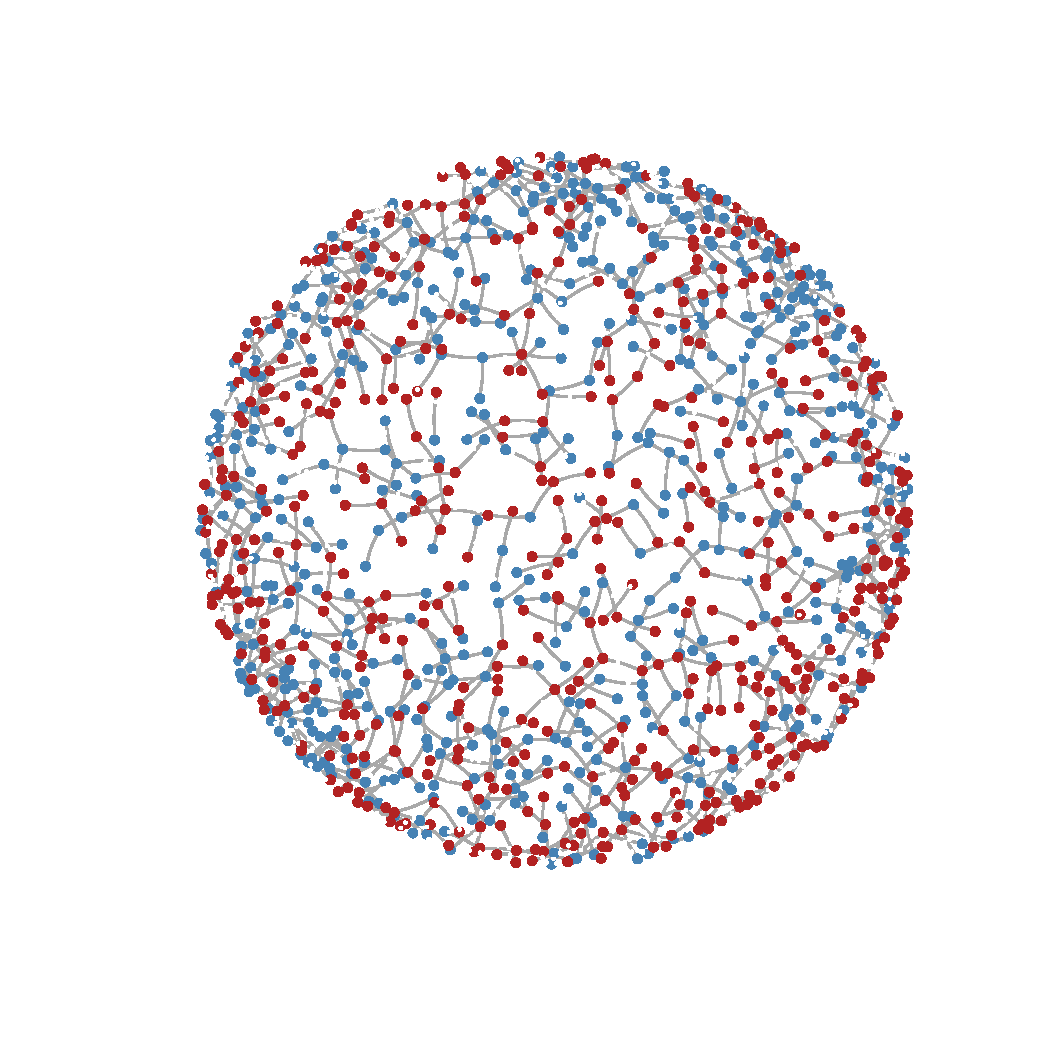
\includegraphics[trim={2cm 2cm 2cm 2cm}, clip, width=\linewidth]{draft/network_plots1.pdf} 
        \caption{Erdos-Renyi random network}
        \label{fig1:random}
    \end{subfigure}
    \hfill
    \begin{subfigure}[t]{0.45\textwidth}
        \centering
        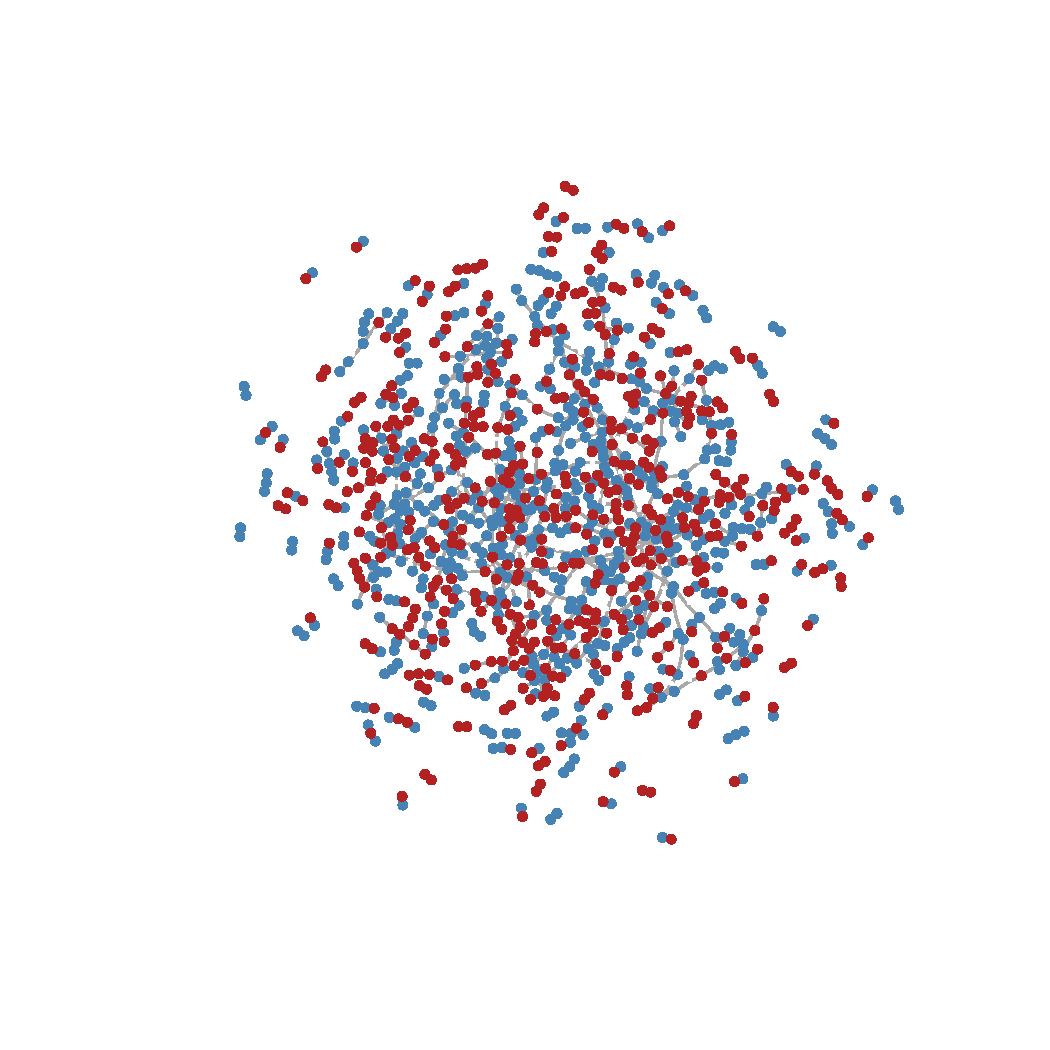
\includegraphics[trim={2cm 2cm 2cm 2cm}, clip, width=\linewidth]{draft/network_plots2.pdf} 
        \caption{Chain network} \label{fig1:tree}
    \end{subfigure}

    \vspace{1cm}
    \begin{subfigure}[t]{0.45\textwidth}
        \centering
        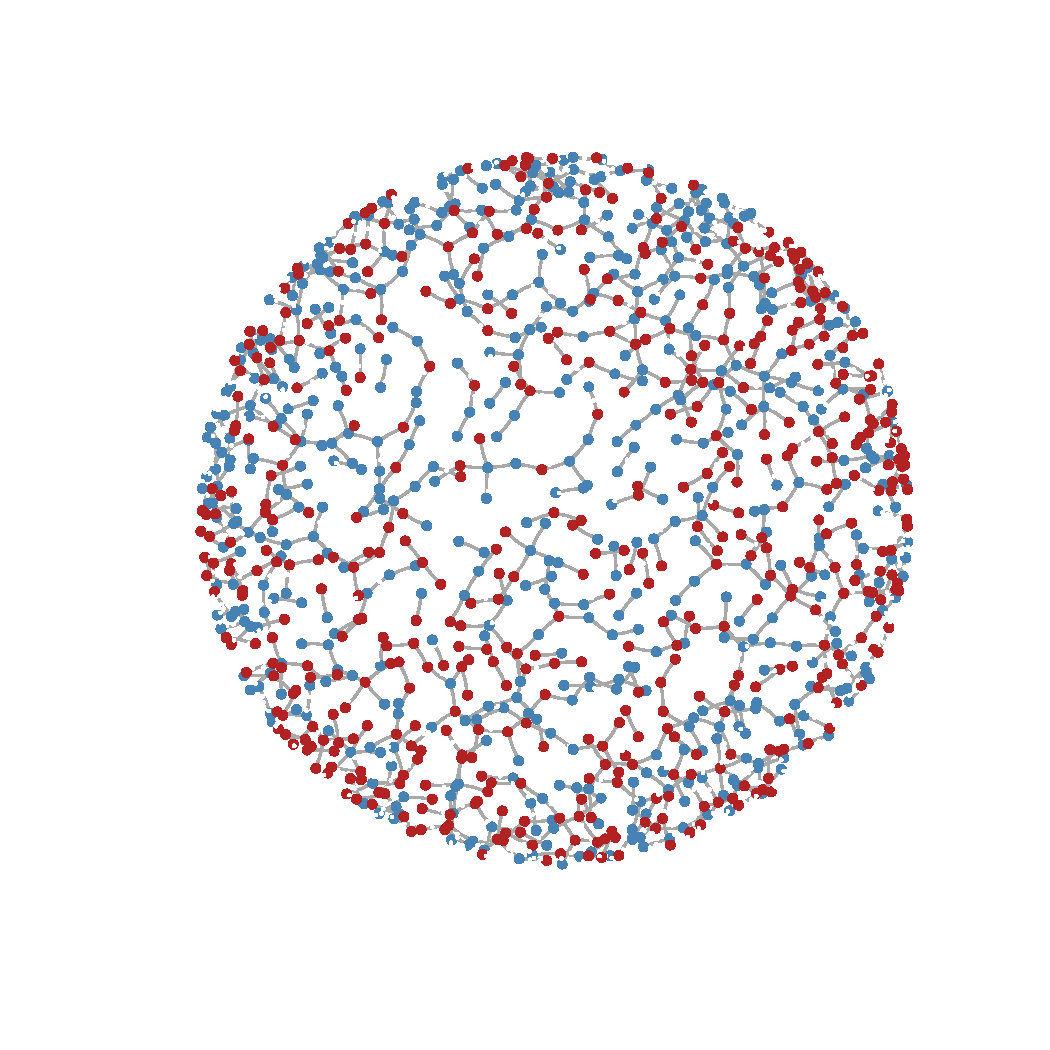
\includegraphics[trim={2cm 2cm 2cm 2cm}, clip, width=\linewidth]{draft/network_plots3.pdf} 
        \caption{Small-world network absent homophily} \label{fig1:nohomophily}
    \end{subfigure}
    \hfill
    \begin{subfigure}[t]{0.45\textwidth}
        \centering
        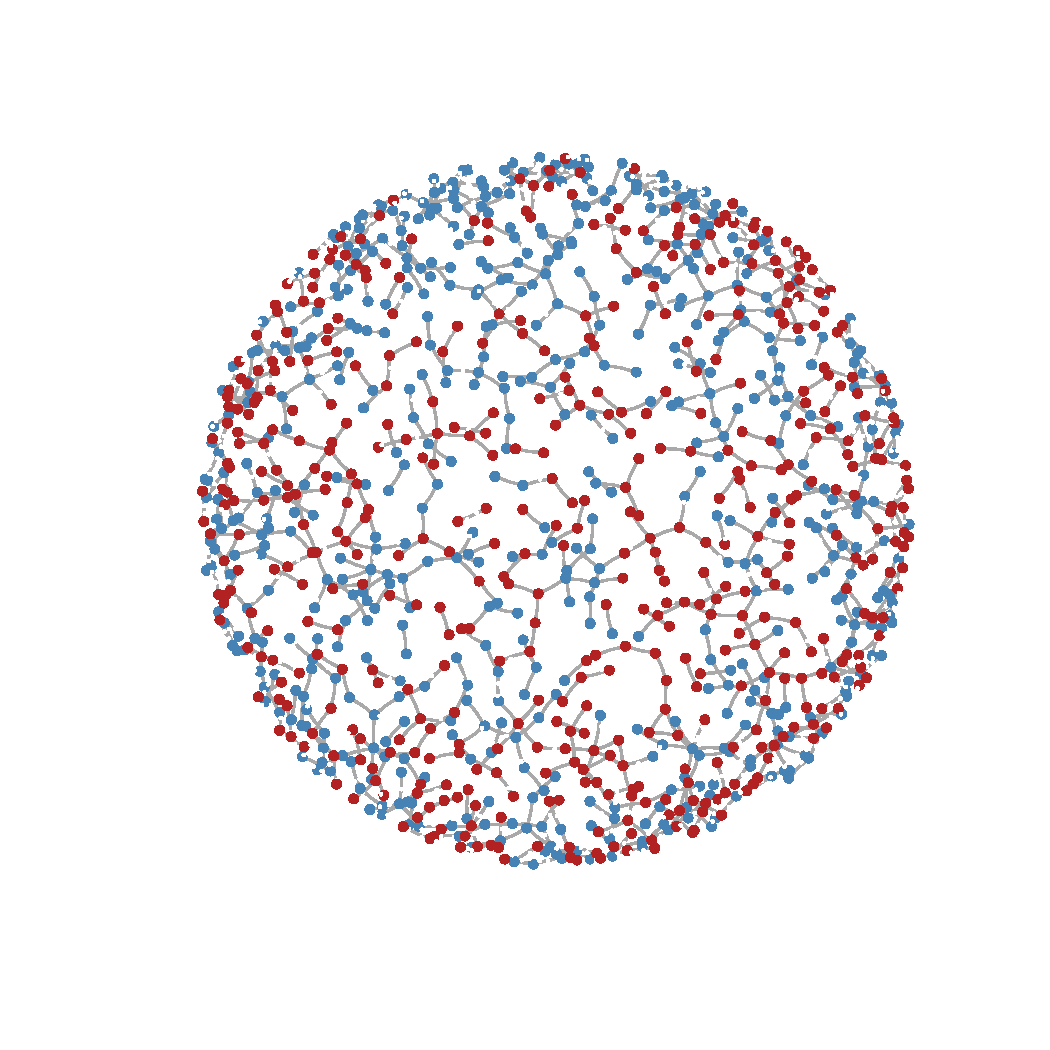
\includegraphics[trim={2cm 2cm 2cm 2cm}, clip, width=\linewidth]{draft/network_plots4.pdf} 
        \caption{Baseline small-world network} \label{fig1:smallworld}
    \end{subfigure}
    
    \vspace{1cm}
    \captionsetup{format=hang}
    \caption{A cross-sectional view of simulated networks from different network topologies. Colored nodes represent nodes that have at least one connection with their neighbor (Red = Republicans, Blue = Democrats) while isolates at given time point was suppressed in visualization. A Erdos-Renyi (ER) random network (a) assumes a homogeneous probability of creating and dropping ties across all nodes conditional on observed density. A chain-like network (b) has more longer chains than the ER random network while lacks triangle-like structure due to constrains on degrees (less than three). While two small-world network has more star-like structure than others, our baseline small-world network (d) is more homophilous than competing specification in (c), as can be seen in Table \ref{tab:Table1}.} \label{fig:Figure1}
\end{figure}    

\subsection{Misinformation Transmission and Progression}

\subsection{Corrective Message Exposure and a Recovery from Misperception}


\printbibliography
%\newpage
%\begingroup
%\parindent 0pt
%\parskip 1ex
%\def\enotesize{\normalsize}
%\theendnotes
%\endgroup
\end{document}
